\documentclass[12pt,a4paper]{article} 
\usepackage[utf8]{inputenx} 
\usepackage[spanish]{babel} 
\usepackage[left=2cm,right=2cm,top=2cm,bottom=2cm]{geometry}
\usepackage{scrextend}
\usepackage{marvosym}
\usepackage{pifont} % Generación de símbolos especiales
\usepackage{textcomp}
\usepackage{newpxtext}
\usepackage{newpxmath}
\usepackage[T1]{fontenc} % Codificación de salida    
\usepackage{microtype} % Mejoras de microtipografía en la obtención de PDF (sólo para pdflatex)
\usepackage[hyphens]{url} % Para escritura de URL
\urlstyle{sf} % Estilo de URL sin serifas para que tengan un mejor aspecto
\usepackage{tikz}
% Paquetes para obtener un mayor control de las listas
\usepackage{paralist} % Mayor control de listas
\usepackage{multicol} % Elementos en varias columnas
\usepackage[breaklinks]{hyperref}
\usepackage{graphicx}
\usepackage{caption}

\usepackage{listings}
\usepackage{color}

\definecolor{dkgreen}{rgb}{0,0.6,0}
\definecolor{gray}{rgb}{0.5,0.5,0.5}
\definecolor{mauve}{rgb}{0.58,0,0.82}

\lstset{frame=tb,
  language=Java,
  aboveskip=3mm,
  belowskip=3mm,
  showstringspaces=false,
  columns=flexible,
  basicstyle={\small\ttfamily},
  numbers=none,
  numberstyle=\tiny\color{gray},
  keywordstyle=\color{blue},
  commentstyle=\color{dkgreen},
  stringstyle=\color{mauve},
  breaklines=true,
  breakatwhitespace=true,
  tabsize=3
}

\captionsetup[figure]{labelformat=empty}
\author{Julián García Sánchez \and Iván Illán Barraya \and Alejandro Medina Jiménez \and Javier Monescillo Buitrón}
\title{Implementación de un procesador de lenguajes para la generación de Autómatas de Moore}
\date{\today}
%%%%%%%%%%%%%%

\begin{document}
	
	\maketitle
	
	\begin{figure}[h]
		\centering
		
\includegraphics[width=0.25
		\linewidth]{img/uclm}
		\caption{}
		\label{fig:image004}
	\end{figure}

	\newpage
	\tableofcontents
	\newpage
	
\section{¿Qué es una máquina de Moore?}
	
En Teoría de la computación un \textbf{autómata} o \textbf{máquina de Moore} es un autómata de estados finitos muy particular, la salida en un momento dado sólo depende de su estado en ese instante, mientras que la transición al siguiente estado dependerá del estado en el que se encuentre y de la entrada introducida.
\newline
	
	\begin{figure}[h]
		\centering
		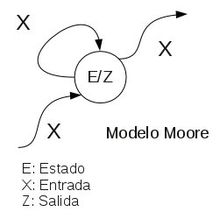
\includegraphics[width=0.5
		\linewidth]{img/modelo-moore}
		\caption{Ejemplo de máquina de Moore simple.}
		\label{fig:modelo-moore}
	\end{figure}
	
Una máquina de Moore \textit{Mmor} se define como una 6-tupla:
	\[ Mmor = (S,S_{0},\Sigma,\Lambda,T,G)  \]
donde definimos los siguientes elementos:
	
	\begin{itemize}
		\item S: es un conjunto finito de estados.
		\item $S_{0}$: es el estado inicial, y además es un elemento de S.
		\item $\Sigma$: un conjunto finito llamado alfabeto de entrada.
		\item $\Lambda$: un conjunto finito llamado alfabeto de salida.
		\item $T$ : una función de transición $T: S \times \Sigma \rightarrow S$ que mapea un estado y una entrada al siguiente estado.
		\item $G$ : una función de salida $G : S \rightarrow \Lambda $ que mapea cada estado al alfabeto de salida.
	\end{itemize}
\clearpage

\newpage

\subsection{Descripción del problema}
El problema que se presenta es la construcción de un procesador de lenguajes cuya entrada consista en un lenguaje de dominio específio en el cuál se declaran una o varias máquinas de Moore. Este lenguaje se ha definido como \textbf{Moor}. La salida del procesador de lenguajes consistirá en uno o varios ficheros generados en un lenguaje de alto nivel. Nosotros hemos elegido \textbf{Java}.

\section{Solución propuesta}
Para diseñar este procesador de lenguajes, utilizaremos los conocimientos de la materia \textit{Procesadores de Lenguajes}durante las distintas etapas del proceso. El proceso consta de 4  etapas:

\begin{itemize}
	\item Diseño del procesador de lenguajes
	\item Analizador Léxico
	\item Analizador Sintáctico
	\item Analizador Semántico
	\item Generación de archivos en lenguaje objeto
\end{itemize}

La primera etapa está más relacionada con lo relacionado al diseño del lenguaje fuente, procesador de lenguajes, o arquitectura. Mediante el uso de diagramas tipo T se explicará el funcionamiento del mismo. Las siguientes tres etapas forman parte de la fase de análisis; mientras que la última etapa forma parte de la fase de síntesis.

\section{Diseño del procesador de lenguajes}

\subsection{Diagramas tipo T}
En primer lugar, se diseña la construcción del procesador de lenguajes empleando los diagramas \textbf{tipo T}. En este diagrama se explica el funcionamiento del procesador que se pretende implementar. Tomamos \textbf{ Moor } como lenguaje fuente, y Java como lenguaje objeto; además el lenguaje que implementa es Java, es decir, nuestro compilador compila a Java, y esta escrito a Java. 
\newline
Para utilizar ese compilador, utilizamos un compilador auxiliar, que está escrito en código máquina para dar lugar a bytecode, el típico archivo \textbf{.class} que generamos al compilar el archivo \textbf{.java}.
\newline
Por último tenemos que compilar el bytecode, con un compilador que acepta bytecode escrito en código máquina. Puede observar este diseño en la siguiente figura.

	\begin{figure}[h]
		\centering
		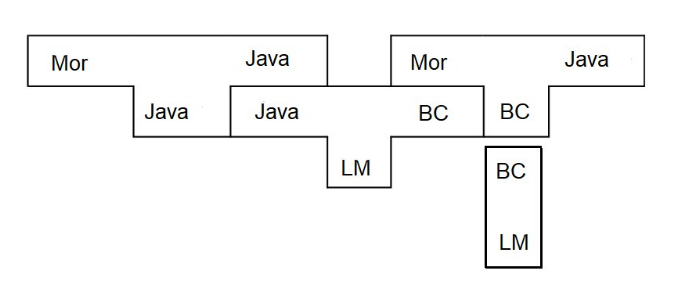
\includegraphics[width=0.5
		\linewidth]{img/T.png}
		\caption{Diagramas tipo T.}
		\label{fig:modelo-moore}
	\end{figure}

\subsection{Lenguaje fuente}
El lenguaje \textbf{Moor} que se ha definido consta de dos secciones principales:

\begin{itemize}
	\item Sección de declaración de código
	\item Sección de declaración de autómatas
\end{itemize}

La \textit{zona de declaración de código} es la parte donde se asignará un comportamiento a un código ya predefinido o que se vaya a ejecutar. Por la forma en la que se ha definido el lenguaje, esta zona será como una zona de \textit{imports} típicamente conocida en lenguajes de alto nivel. 
\newline
\newline
La estructura de esta zona es: c$N$ $\#$ \textit{código} $\#$ donde c es el comportamiento, $N$ es el número de comportamiento y los \textbf{tokens} $\#$ son los delimitadores del código. \newline La característica principal de esta zona es que solo se podrán realizar este tipo de declaraciones, ya que en la otra zona solo podremos declarar autómatas.

\begin{center}
	Ejemplo : c1 $\#$ print('hola') $\#$
\end{center}

Respecto a la \textit{zona de declaración de autómatas} se tendrá una serie de palabras que se utilizarán para la definición del autómata. No obstante en esta zona solo se podrán declarar autómatas y las funciones asociadas a los mismos, también, como en cualquier lenguaje de alto nivel, se podrán incluir los clásicos comentarios '//' o '/$\ast$ Texto comentario '$\ast$/'.
\newline 
\newline
Será posible la declaración de múltiples autómatas en el fichero de prueba, además, se indicará en una tabla todos los campos que son imprescindibles para la realización del mismo.
Cualquier otro carácter introducido en el fichero de prueba será considerado como error.

\subsection{Tabla de Token-Acción}
Primero, presentamos la tabla Token-Acción. En esta tabla se describen tanto los tokens que componen nuestro lenguaje, como la función de cada uno de ellos.

\begin{center}
\begin{tabular}{|c|c|}
	\hline 
	\textbf{Token} & \textbf{Acción} \\ 
	\hline 
	moore & Función para declarar un autómata seguido de un nombre   \\
	& que se escribirá entre llaves $\{\}$ moore Ejemplo $\{\}$\\
	\hline 
	estados & Indica la cantidad de estados totales que tendrá el autómata  \\
	& puede ser un único estado o varios separados por ',' estados q0,q1;\\ 
	\hline 
	estado\_in & Se selecciona un único estado inicial  \\ 
	& que tendrá que estar en los estados anteriores estado\_in q0; \\
	\hline 
	alf\_in & La entrada o eventos del autómata que hará posible las transiciones\\
	& entre estados, único o entre comas ',' alf\_in a,b,c;\\
	\hline 
	alf\_out &  La salida o comportamientos del autómata  \\
	& y tendrán que ser coincidentes con \\ 
	& la zona de declaración de comportamientos, \\
	&  escrito un identificador único o entre comas ',' \\
	\hline
	transicion & Será un tipo de función que se escribirá entre llaves $\{\}$, \\
	& y permitirá que se transite mediante una entrada de un estado a otro: \\ 
	& (<estado\_origen>, entrada, <estado\_destino>); \\
	& se podrán indicar varias mediante el uso de comas ',' \\
	\hline 
	comportamiento & Será un tipo de función que se escribirá entre llaves $\{\}$,   \\ 
	& y permite asignar a un estado un comportamiento: \\
	& (<estados>,<comportamiento>); \\
	& se podrán indicar varios mediante el uso de comas ','\\
	\hline  
\end{tabular} 
\end{center}
Notese, que para cerrar una sentencia es necesario de indicar al final de dicha sentencia el carácter ';', esto no es necesario para las funciones \textit{moore}, \textit{transicion} y \textit{comportamiento}.
\newline

\subsection{Tabla de tokens}
En segundo lugar, creamos la tabla de tokens, dónde también mostramos lexemas de ejemplo y los patrones asociados a cada token.
\begin{center}
		\begin{tabular}{|c|c|c|}
			\hline 
			\textbf{Token} & \textbf{Lexema} & \textbf{Patrón} \\ 
			\hline 
			moore & moore & m$\cdot$o$\cdot$o$\cdot$r$\cdot$e  \\ 
			\hline 
			estados &estados & e$\cdot$s$\cdot$t$\cdot$a$\cdot$d$\cdot$o$\cdot$s \\ 
			\hline 
			estado$\_$in & estado$\_$in & e$\cdot$s$\cdot$t$\cdot$a$\cdot$d$\cdot$o$\cdot$$\_$$\cdot$i$\cdot$n \\ 
			\hline 
			alf$\_$in	& alf$\_$in & a$\cdot$l$\cdot$f$\cdot$$\_$i$\cdot$n \\ 
			\hline 
				alf$\_$out	& alf$\_$out & a$\cdot$l$\cdot$f$\cdot$$\_$o$\cdot$u$\cdot$t \\ 
			\hline 
				transicion	& transicion & t$\cdot$r$\cdot$a$\cdot$n$\cdot$s$\cdot$i$\cdot$c$\cdot$i$\cdot$o$\cdot$n \\ 
			\hline 
				comportamiento	& comportamiento & c$\cdot$o$\cdot$m$\cdot$p$\cdot$o$\cdot$r$\cdot$t$\cdot$a$\cdot$m$\cdot$i$\cdot$e$\cdot$n$\cdot$t$\cdot$o \\ 
			\hline 
			Paréntesis abierto	& ( & ( \\ 
			\hline 
			Paréntesis cerrado	& ) & ) \\ 
			\hline 
			Llave abierta	& $\{$ & $\{$ \\ 
			\hline 
			Llave cerrada	& $\}$ & $\}$ \\ 
			\hline 
			Punto y coma	& ; & ; \\ 
			\hline 
			Coma	& , &  , \\ 
			\hline
			Asterisco barra & $\ast/$  & $\ast$$\cdot/$ \\ 
			\hline 
			Barra asterisco & $/\ast$  &  $/$$\cdot$$\ast$ \\ 
			\hline  
			ID	& hola  & [A-Za-z][A-Zaz0-9$\_$]* \\ 
			\hline 
			CMP	& c1 & c[1-9][0-9]* \\ 
			\hline
		    CODIGO	& $\#$codigo aquí $\#$  & $\#$$\cdot$ codigo aquí $\cdot$$\#$\\ 
			\hline
		\end{tabular} 	
	\end{center}
\clearpage

\subsection{EBNF}
Por último, en la siguiente figura puede ver una representación de las expresiones regulares que definen el léxico de nuestro lenguaje en EBNF; el metalenguaje que hemos estudiado durante la asignatura.

			\begin{center}
			\begin{tabular}{lcl}
	

				PROGRAMA & ::= & DEC$\_$COMP AUTOMATA $\{$AUTOMATA$\}$ \\ 
				 
				
				DEC$\_$COMP & ::= &CMP  CODIGO $\{$ CMP CODIGO $\}$ \\ 
			
				CODIGO 	&::= &'$\#$' ASCII '$\#$' \\ 
				
				AUTOMATA & ::= & \textbf{moore} ID CUERPO$\_$AUTOMATA \\
				
			
				CUERPO$\_$AUTOMATA	& ::= & $'\{'$ ESTADOS ESTADO$\_$INI ALF$\_$IN  \\ 
				
					& &  ALF$\_$OUT TRANSICION COMPORTAMIENTOS $'\}'$ \\ 
				
				ESTADOS	& ::= &   \textbf{estados} $\{$ ID ',' $\}$ ID ';'\\ 
				
				 ESTADO$\_$INI &::= & \textbf{estado$\_$in} ID ';'\\ 
				 
				ALF$\_$IN &::= & \textbf{alf$\_$in}  $\{$ EVENTOS ',' $\}$ EVENTOS ';' \\ 
				
				ALF$\_$OUT & ::= &\textbf{alf$\_$out}  $\{$ CMP ',' $\}$ CMP ';'  \\ 
				
				TRANSICION 	 & ::= & \textbf{transicion} $'\{'$ TRANSICION$\_$DEF $\{$ ',' TRANSICION$\_$DEF  $\}$ ';' $'\}'$ \\ 
				
				TRANSICION$\_$DEF & ::= & '(' ID ',' ID ',' ID ')' \\ 
			
				
				COMPORTAMIENTOS	 & ::= &  \textbf{comportamientos} $'\{'$ COMP$\_$DEF $\{$ ',' COMP$\_$DEF $\}$ ';' $'\}'$\\ 
				
				COMP$\_$DEF &  ::= & '(' ID ',' ID ',' ID ')' \\ 
				
				
				CMP  & ::= & 'c'NUMEROS \\ 
				
				NUMEROS &::= & 0 | 1 | .. | 9 \\ 
				
				COMENTARIOS & ::=  & $'/\ast'$ ASCII $'\ast/'$ \\
				
				
			\end{tabular} 	
		\end{center}
	
	\clearpage

\section{Analizador Léxico}
El analizador léxico tiene varias funciones:
\begin{itemize}
	\item Reconocer los símbolos / tokens que componen el texto fuente.
	\item Eliminar comentarios del texto fuente.
	\item Eliminar espacios en blanco, saltos de línea, tabulaciones, etc.
	\item Informar de los errores léxicos detectados
\end{itemize}

Como salida del analizador léxico, se obtiene una representación de la cadena de entrada en forma de cadena de tokens, que será posteriormente utilizada en la fase de análisis sintáctico. Para construir el analizador sintáctico hemos utilizado dos herramientas: JFlex y ANTLR. 
Por un lado, JFlex es una herramienta software en la que se declaran los tokens que componen nuestro lenguaje fuente, así como las expresiones regulares asociadas a los mismos; y genera una serie de archivos que cumplen la función del analizador léxico. 
Por otro lado, ANTLR Jarillo.	
\subsection{Jflex}

En esta sección se muestra el código en JFlex donde se construye el analizador léxico del lenguaje Moor.

\begin{lstlisting}[caption=Analizador Léxico en JFlex]

//* --------------------------Seccion codigo-usuario ------------------------*/
package plmoore;
import java.util.*;
import java.io.*;
import java_cup.runtime.Symbol;

%%


/* -----------------Seccion de opciones y declaraciones -----------------*/

/*--OPCIONES --*/

%class AnalizadorAutomata
%unicode
%cup
%cupdebug
%ignorecase

/* Posibilitar acceso a la columna y fila actual de analisis*/

%line
%column


/*--DECLARACIONES --*/

%{

%}

%init{
	System.out.println("Iniciando Analizador Lexico ... ");

%init}


%eof{

	System.out.println("Fin del Analizador Lexico ... ");

%eof}

TERLINEA = \r|\n|\r\n
CARACTERIN = [^\r\n]
ESPACIOBLANCO = {TERLINEA} | [ \t\f]
COMENTARIO = {COMENTARIOTRADICIONAL} | {FINLINEACOMENT}
COMENTARIOTRADICIONAL   = "/*" [^*] ~"*/" | "/*" "*"+ "/"
FINLINEACOMENT     = "//" {CARACTERIN}* {TERLINEA}?
ENTEROS = 0 | [1-9][0-9]*
CMP = c{ENTEROS}
ESTADOS = "estados"
EINICIAL = "estado_in"
ALF_OUT = "alf_out"
ALF_IN = "alf_in"
TRANS = "transicion"
COMPORT = "comportamiento"
ID = [:jletter:] [:jletterdigit:]*
MOORE = "moore"

%state CODIGO

%%

/* ------------------------Seccion de reglas y acciones ----------------------*/

<YYINITIAL> {

	{CMP} { return new Symbol(sym.CMP, yyline, yycolumn, new String(yytext())); }
	"#" {yybegin(CODIGO); return new Symbol(sym.ALM_OP, yyline, yycolumn, new String(yytext())); }
	{MOORE} { return new Symbol(sym.MOORE, yyline, yycolumn, new String(yytext()));}
	"{" { return new Symbol(sym.LLCORCH_OP, yyline, yycolumn, new String(yytext()));}
	"}" { return new Symbol(sym.LLCORCH_CL, yyline, yycolumn, new String(yytext()));}
	{ESTADOS} { return new Symbol(sym.ESTADOS, yyline, yycolumn, new String(yytext()));}
	{EINICIAL} { return new Symbol(sym.ESTADO_INI, yyline, yycolumn, new String(yytext()));}
	{ALF_IN}  { return new Symbol(sym.ALF_IN, yyline, yycolumn, new String(yytext()));}
	{ALF_OUT} { return new Symbol(sym.ALF_OUT, yyline, yycolumn, new String(yytext()));}
	{TRANS}   {  return new Symbol(sym.TRANS, yyline, yycolumn, new String(yytext()));}
	{COMPORT} { return new Symbol(sym.COMPORTAMIENTO, yyline, yycolumn, new String(yytext()));}
	"," { return new Symbol(sym.COMA, yyline, yycolumn, new String(yytext()));}
	";" { return new Symbol(sym.PUNTO_COMA, yyline, yycolumn, new String(yytext()));}
	"(" { return new Symbol(sym.LLPARENT_OP, yyline, yycolumn, new String(yytext()));}
	")" { return new Symbol(sym.LLPARENT_CL, yyline, yycolumn, new String(yytext()));}
	{ID} {return new Symbol(sym.ID, yyline, yycolumn, new String(yytext()));}
	{COMENTARIO}                      {/*Se ignoran los comentarios */}
	{ESPACIOBLANCO}                   {/*Se ignoran los espacios en blanco */}	
}

<CODIGO>{
	. + /"#" { return new Symbol(sym.CODIGO, yyline, yycolumn, new String(yytext()));}
	"#" { yybegin(YYINITIAL); return new Symbol(sym.ALM_CL, yyline, yycolumn, new String(yytext()));}
}

[^]            { String errLex = "Error lexico : '"+yytext()+"' en la linea: "+(yyline+1)+" y columna: "+(yycolumn+1);
		 System.out.println(errLex); }

\end{lstlisting}

\subsection{ANTLR}

Jarillo

\section{Analizador sintáctico}
El analizador sintáctico tiene varias funciones:
\begin{itemize}
	\item Analizar la secuencia de tokens y verificar si son correctos sintácticamente.
	\item Obtener una representación interna del texto.
	\item Informar de los errores sintácticos detectados.
\end{itemize}
En resumen, dada la cadena de tokens ontenida como resultado de la fase de análisis léxico, se compruena que dicha secuencia está escrita correctamente; y se obtiene una representación interna de la misma, que servirá como entrada para el proceso de análisis semántico. 

Como sabemos, existen dos formas de realizar el análisis sintáctico (ascendente y descendente). Nosotros hemos escogido construir un analizador sintáctico ascendente con CUP y ANTLR. 

Por un lado, CUP es una herramienta que hemos utilizado durante las prácticas de la asignatura; y que permite declarar las producciones que constituyen las reglas sintácticas del lenguaje fuente; además de reglas semánticas asociadas a las mismas, que se tratarán en más detalle en la siguiente sección. 

En la sección "Archivo Cup" puede ver el código asociado a esta fase de la construcción del procesador de lenguajes.

\subsection{Control de errores en cup}

Para controlar los errores sintácticos en CUP, se han utilizado producciones de error. Las producciones de error utilizan un símbolo terminal "error"; de tal manera que cuando se produce una reducción al mismo, se invoque a una rutina de error asociada a este símbolo. En esta rutina de error, se invoca al método report\_error de la clase Parser.

En la sección "Archivo Cup" puede ver el código asociado a esta fase de la construcción del procesador de lenguajes.

\subsection{Antlr}

Jarillo.

\section{Analizador semántico}

El analizador semántico tiene varias funciones:

\begin{itemize}
	\item Dar significado a las construcciones del lenguaje fuente. 
	\item Generación de código.
	\item Acabar de completar el lenguaje fuente.
\end{itemize}
 
La tercera función del analizador semántico tiene que ver con aspectos como controlar que la cadena introducida esté formada por elementos del alfabeto de entrada, que los estados que se declaren en la máquina de Moore sean los únicos a los que se puede transitar, o que no se declare varias veces una transición; entre otros aspectos.

Medina - Esto de abajo lo puedes usar, o no. Lo que tú quieras

Para controlar este tipo de errores, se han introducido reglas semánticas en las producciones declaradas en el archivo CUP mencionado en la sección anterior. En estas reglas se controlan todos los aspectos mencionados con anterioridad, además de añadir funcionalidad al código generado. Es decir, este conjunto de reglas semánticas no solo tienen el propósito de completar el lenguaje fuente, sino de dar funcionalidad a la máquina (o máquinas) de Moore que se declaran en el mismo.

En la sección "Archivo Cup" puede ver el código asociado a esta fase de la construcción del procesador de lenguajes.

\subsection{ANTLR}

\subsection{Generación de código}

Javier

\section{Archivo Cup}

En este archivo se muestran tanto las producciones asociadas a la gramática y utilizadas para realizar el análisis sintáctico, como las reglas semánticas asociadas a cada producción; que permiten el análisis semántico. 

\begin{lstlisting}[caption=Analizador Sintáctico y Semántico en CUP]

/* ----------------------Seccion de declaraciones package e imports--------------------*/
package plmoore;

import java.io.*;
import java_cup.runtime.*;
import java.util.ArrayList;
import java.util.Hashtable;

/* ----------------------Seccion componentes de codigo de usuario --------------------*/
parser code {:


	public void report_error(String message, Object info) {
   
        /* Crea un StringBuffer llamado 'm' con el string 'Error' en el. */

        StringBuffer m = new StringBuffer("Error");
   
        /* Chequea si la informacion pasada al metodo es del mismo
           tipo que el tipo java_cup.runtime.Symbol. */

        if (info instanceof java_cup.runtime.Symbol) {

            /* Declara un objeto 's' del tipo java_cup.runtime.Symbol con la
               informacion que hay en el objeto info que esta siendo convertido
               como un objeto java_cup.runtime.Symbol. */
            java_cup.runtime.Symbol s = ((java_cup.runtime.Symbol) info);
   
            /* Chequea si el numero de linea en la entrada es mayor o
               igual que cero. */
            if (s.left >= 0) {                
                /* Anade al final del mensaje de error StringBuffer
                   el numero de linea del error en la entrada. */
                m.append(" en la linea "+(s.left+1));   
                /* Chequea si el numero de columna en la entrada es mayor
                   o igual que cero. */
                if (s.right >= 0)                    
                    /* Anade al final del mensaje de error StringBuffer
                       el numero de columna del error en la entrada. */
                    m.append(", columna "+(s.right+1));
            }
        }
        /* Anade al final del mensaje de error StringBuffer creado en
           este metodo el mensaje que fue pasado a este metodo. */
        m.append(" : "+message);
   
        /* Imprime los contenidos del StringBuffer 'm', que contiene
           el mensaje de error. */
        System.err.println(m);
    }
    public void report_fatal_error(String message, Object info) {
        report_error(message, info);
        System.exit(1);
    }

    public void syntax_error(Symbol s){
        System.out.println("Error recuperable de sintaxis: "+s.value+" Linea "+(s.left+1)+" columna "+(s.right+1) );
    }

    public void unrecovered_syntax_error(Symbol s) throws java.lang.Exception{ 
        System.out.println("Error no recuperable de sintaxis: "+s.value+" Linea "+(s.left+1)+" columna "+(s.right+1) );
    }

   
:}

action code {: 

	MoldeAutomataMoore machine;
	int contador = 0;
        ArrayList<MoldeAutomataMoore> maquinas = new ArrayList<MoldeAutomataMoore>();;
	Hashtable<String, String> comp_codigo = new Hashtable<String, String>();
        String fallos_ejecucion = "";
        boolean continuar = true;
:}

/* ------------Declaracion de la lista de simbolos de la gramatica-----------*/
non terminal programa, dec_comp, dec_automata, cuerpo_automata, estados, dec_estados, estado_ini, alf_in, dec_alf_in, alf_out, dec_alf_out, transicion, dec_transicion, comportamientos, dec_comportamientos;
non terminal MoldeAutomataMoore automata;
non terminal String codigo, comp_def, transicion_def;


terminal String CMP, CODIGO, MOORE, ID, LLCORCH_OP, LLCORCH_CL, ESTADOS, ESTADO_INI, ALF_IN, ALF_OUT, TRANS, COMPORTAMIENTO, COMA, PUNTO_COMA, LLPARENT_OP, LLPARENT_CL, ALM_OP, ALM_CL;


/* --------------Declaracion de la gramatica -----------*/

programa ::= dec_comp dec_automata {: 

        System.out.println("Analisis finalizado"); 
        if(continuar){
           System.out.println("Generando fichero...");
           GeneracionCodigo generar = new GeneracionCodigo(maquinas);
           
        }else{
           System.out.println("Hubo fallos durante la ejecucion"); 
           System.out.println(fallos_ejecucion);
        }

                                    :} ;

dec_comp ::= CMP:com codigo:code {: comp_codigo.put(com, code); :} dec_comp
		| CMP:com codigo:code {: comp_codigo.put(com, code); :} ;

dec_automata ::= automata:machin {: 
                                    System.out.println("Maquina identificada! n_maquinas: "+ ++contador); maquinas.add(machin); 
                                  :} dec_automata

		| automata:machin {: 
                                    System.out.println("Maquina identificada! n_maquinas: "+ ++contador); maquinas.add(machin); 
                                   :};

codigo ::= ALM_OP CODIGO:code ALM_CL {: RESULT=code; :} 
		   | error {:
				fallos_ejecucion += " Error declarando codigo de usuario\n";
				parser.report_error(fallos_ejecucion,null);
				continuar = false;
		   :};


automata ::= MOORE ID:id {: machine = new MoldeAutomataMoore(id); :} cuerpo_automata {: RESULT = machine; :}
		   | error {:
				fallos_ejecucion += " Error declarando maquina de Moore\n";
				parser.report_error(fallos_ejecucion,null);
				continuar = false;
		   :};


cuerpo_automata ::= LLCORCH_OP estados estado_ini alf_in alf_out comportamientos transicion LLCORCH_CL 
		   | error {:
				fallos_ejecucion += " Error declarando maquina de Moore\n";
				parser.report_error(fallos_ejecucion,null);
				continuar = false;
		   :};

estados ::=  ESTADOS dec_estados PUNTO_COMA 
		   | error {:
				fallos_ejecucion += " Error declarando estados\n";
				parser.report_error(fallos_ejecucion,null);
				continuar = false;
		   :}; 

dec_estados ::= ID:id {: 
                            if(!machine.addEstado(id)){
fallos_ejecucion += "In line: "+((idleft)+1)+" El estado "+id+" ya esta declarado \n"; continuar = false;} 

                       :} COMA dec_estados

	        | ID:id {: 
                            if(!machine.addEstado(id)){fallos_ejecucion += "In line: "+((idleft)+1)+" El estado "+id+" ya esta declarado \n"; continuar = false;} 
                         :} ;

             

estado_ini ::= ESTADO_INI ID:id {: machine.setEstado_inicial(id); :} PUNTO_COMA 
		   | error {:
				fallos_ejecucion += " Error declarando estado inicial\n";
				parser.report_error(fallos_ejecucion,null);
				continuar = false;
		   :};
         

alf_in ::= ALF_IN dec_alf_in PUNTO_COMA 
		   | error {:
				fallos_ejecucion += " Error declarando alfabeto de entrada\n";
				parser.report_error(fallos_ejecucion,null);
				continuar = false;
		   :};

dec_alf_in ::= ID:id {: if(!machine.addEvento(id)){fallos_ejecucion += "In line: "+((idleft)+1)+" El evento "+id+" ya esta declarado \n"; continuar = false;} 

                      :} COMA dec_alf_in

		| ID:id {: if(!machine.addEvento(id)){fallos_ejecucion += "In line: "+((idleft)+1)+" El evento "+id+" ya esta declarado \n"; continuar = false;} 
                         :} ;

alf_out ::= ALF_OUT dec_alf_out PUNTO_COMA 
		   | error {:
				fallos_ejecucion += " Error declarando alfabeto de salida\n";
				parser.report_error(fallos_ejecucion,null);
				continuar = false;
		   :};

dec_alf_out ::= CMP:id {: if(!machine.addComp(id)){fallos_ejecucion += "In line: "+((idleft)+1)+" El comportamiento "+id+" ya esta declarado \n"; continuar = false;} 

                        :} COMA dec_alf_out

		| CMP:id {: if(!machine.addComp(id)){fallos_ejecucion += "In line: "+((idleft)+1)+" El comportamiento "+id+" ya esta declarado \n"; continuar = false;} 
                          :} ;

comportamientos ::= COMPORTAMIENTO LLCORCH_OP dec_comportamientos PUNTO_COMA LLCORCH_CL 
		   | error {:
				fallos_ejecucion += " Error declarando alfabeto de comportamientos\n";
				parser.report_error(fallos_ejecucion,null);
				continuar = false;
		   :};

dec_comportamientos ::= comp_def:tupla {: boolean error = machine.addComportamiento(tupla);

                    if(!error){ fallos_ejecucion += "In line: "+((tuplaleft)+1)+" El comportamiento "+tupla+" ya esta declarado \n"; continuar = false; }

                                        :} COMA dec_comportamientos 

                    | comp_def:tupla {: boolean error = machine.addComportamiento(tupla);
                       if(!error){ fallos_ejecucion += "In line: "+((tuplaleft)+1)+" El comportamiento "+tupla+" ya esta declarado \n"; continuar = false; }
                                      :} ;

comp_def ::= LLPARENT_OP ID:id COMA CMP:comp LLPARENT_CL {: RESULT=id+"-"+comp+"-"+comp_codigo.get(comp); :}
		   | error {:
				fallos_ejecucion += " Error declarando alfabeto comportamientos\n";
				parser.report_error(fallos_ejecucion,null);
				continuar = false;
		   :};

transicion ::= TRANS LLCORCH_OP dec_transicion PUNTO_COMA LLCORCH_CL 
		   | error {:
				fallos_ejecucion += " Error declarando alfabeto de transiciones\n";
				parser.report_error(fallos_ejecucion,null);
				continuar = false;
		   :};

dec_transicion ::= transicion_def:tupla {:  if(!machine.addTransicion(tupla)){
                                              fallos_ejecucion += "In line: "+((tuplaleft)+1)+" El comportamiento "+tupla+" ya esta declarado \n"; 
                                              continuar = false; }
                                        :} COMA dec_transicion 

		| transicion_def:tupla {:  if(!machine.addTransicion(tupla)){
                                              fallos_ejecucion += "In line: "+((tuplaleft)+1)+" El comportamiento "+tupla+" ya esta declarado \n"; continuar = false; }
                                        :} ;

transicion_def ::= LLPARENT_OP ID:estado_in COMA ID:evento COMA ID:estado_out LLPARENT_CL {: RESULT=estado_in+"-"+evento+"-"+estado_out; :} ;
	





\end{lstlisting}


\section{Bibliografía}
	\clearpage
	
	\begin{thebibliography}{99}
		\bibitem{Moore1} Autómatas de Moore \url{https://es.wikipedia.org/wiki/M%C3%A1quina_de_Moore}
	
	\end{thebibliography}	
	
\end{document}\grid
